\documentclass[a5paper,12pt,twoside]{book}

\usepackage[tmargin=20mm,bmargin=25mm,lmargin=20mm,rmargin=20mm]{geometry} % Formato de página

\usepackage[output-decimal-marker={,}]{siunitx} % Unidades del SI
    \sisetup{per-mode = fraction}
    \DeclareSIUnit{\rpm}{rpm}
    \DeclareSIUnit{\atmosphere}{atm}

\usepackage[framemethod=TikZ]{mdframed} % Define \begin{mdframed}[style=MyFrame1]

    \mdfdefinestyle{MyFrame1}
    {linecolor=black!80!gray,
    outerlinewidth=0.5pt,
    roundcorner=0pt,
    innertopmargin=15pt,
    innerbottommargin=20pt,
    innerrightmargin=15pt,
    innerleftmargin=15pt,
    backgroundcolor=gray!30!white}

    \mdfdefinestyle{MyFrame2}
    {linecolor=white,
    outerlinewidth=0.5pt,
    roundcorner=10pt,
    innertopmargin=15pt,
    innerbottommargin=20pt,
    innerrightmargin=15pt,
    innerleftmargin=15pt,
    backgroundcolor=gray!20!white}

\usepackage{graphicx}
    \graphicspath{{./images/}} % Define \graphicspath{{dir1}{dir2}} para incluir imágenes que estén en los directorios dir1 y dir2

\usepackage[spanish]{babel}  % Traducciones y abreviaturas
\usepackage{amssymb}  % Símbolos y tipografía matemáticos
\usepackage{amsmath}  % Formato y estructura matemáticos
\usepackage{esint} % Define \oiint para integrales cerradas y acomoda \iiint
\usepackage{hyperref}  % Referencias cruzadas
\usepackage{fancyhdr}  % Encabezado y pie
\usepackage{graphicx}  % Define \includegraphics
\usepackage{pdfpages} % Define \includepdf
\usepackage{comment} % Comenta todo entre \begin{comment} \end{comment}
% COMANDOS DE FORMATO
\newcommand{\sub}[2]{{{#1}_\textsl{{#2}}}} % #1 subíndice #2 (Usado cuando #2 es $texto$)
\newcommand{\scale}[2]{\text{\scalebox{#1}{$#2$}}} % Aplicar factor de escala #1 a la ecuación #2
\newcommand{\cusTi}[1]{\noindent\textbf{#1}} % Título de definiciones, propiedades y ejemplos
\newcommand{\cusTe}[1]{\vspace{2mm}\\\text{\hspace{\the\parindent}}#1} % Descripción de definiciones, propiedades y ejemplos
\newcommand{\noTi}[1]{\text{\hspace{\the\parindent}}#1} % Descripción de MyFrame1 que no tenga título
\newcommand{\concept}[1]{\vspace{1ex} \textsc{#1}} % Subtítulos sin jerarquía
\newcommand{\braces}[1]{{ \left\{ {#1} \right\} }} % #1 entre llaves
\newcommand{\sqb}[1]{{ \begin{bmatrix} #1 \end{bmatrix} }} % #1 entre corchetes
\newcommand{\bb}[1]{\left(#1\right)} % #1 entre paréntesis
\newcommand{\sfrac}[2]{#1/#2} % Fracciones #1/#2 para reemplazar el (muy lento) \usepackage{xfrac}
\newcommand{\captionSpace}{-0.8cm} % Espacio entre figuras y pie de foto

% COMANDOS PARA NOTACIÓN DE FUNCIONES
\newcommand{\barrow}[3]{\begin{bmatrix} \left. #1 \right|_{#2}^{#3} \end{bmatrix}} % Regla de Barrow de #1 para los extremos de integración #2 y #3
\newcommand{\fx}[2][f]{#1 \hspace{-0.5mm} \left( #2 \right)} % #1 en función de #2 con paréntesis
\newcommand{\ffx}[2][f]{#1 \hspace{-0.5mm} \begin{bmatrix} #2 \end{bmatrix}} % #1 en función de #2 con corchetes
\newcommand{\intProd}[2]{<\hspace{-0.8mm}#1,#2\hspace{-0.8mm}>} % Producto interno entre #1 y #2
\newcommand{\comb}[2]{\begin{pmatrix} {#1}\\{#2} \end{pmatrix}} % Combinatorio n=#1, m=#2
\newcommand{\media}[2]{\underset{#2}{\sub{#1}{med}}} % #1 media entre #2
\newcommand{\norm}[1]{{\left| {#1} \right|}} % Módulo de #1
\newcommand{\nnorm}[1]{{\left|\left| {#1} \right|\right|}} % Norma de #1
\newcommand{\trans}[1]{#1^*} % Matriz transpuesta de #1
\newcommand{\conj}[1]{\overline{#1}} % Conjugado de #1
\newcommand{\ave}[1]{\bar{#1}} % Valor promedio de #1
\newcommand{\rms}[1]{{\sub{#1}{ef}}} % Valor eficaz de #1
\newcommand{\peak}[1]{{\sub{#1}{pk}}} % Valor pico de #1

% COMANDOS PARA NOTACIÓN DE ELEMENTOS Y OPERADORES
\newcommand{\class}[1][1]{\mathcal{C}^{#1}} % Clase o cantidad de derivadas parciales contínuas
\newcommand{\versor}[1]{\hat{#1}} % Vector unitario #1
\newcommand{\fasor}[1]{\check{#1}} % Fasor #1
\newcommand{\iVer}{\versor{\imath}} % i versor
\newcommand{\jVer}{\versor{\jmath}} % j versor
\newcommand{\kVer}{\versor{k}} % k versor
\newcommand{\eVer}{\versor{\textbf{e}}} % Versor canónico
\newcommand{\tang}{\textbf{t}} % Vector tangente
\newcommand{\setO}{\varnothing} % Conjunto vacío
\newcommand{\setN}{\mathbb{N}} % Conjunto de los números naturales
\newcommand{\setZ}{\mathbb{Z}} % Conjunto de los números enteros
\newcommand{\setR}{\mathbb{R}} % Conjunto de los números reales
\newcommand{\setI}{\mathbb{I}} % Conjunto de los números imaginarios
\newcommand{\setC}{\mathbb{C}} % Conjunto de los números complejos
\newcommand{\iu}{\mathrm{i}\mkern1mu} % Unidad imaginaria o número i
\newcommand{\setV}{\mathbb{V}} % Espacio vectorial V
\newcommand{\setW}{\mathbb{W}} % Espacio vectorial W
\newcommand{\setK}{\mathbb{K}} % Cuerpo K
\newcommand{\ith}{i} % Valor i-ésimo para sumatorias y permutadores
\newcommand{\jth}{j} % Valor j-ésimo para sumatorias y permutadores
\newcommand{\kth}{k} % Valor k-ésimo para sumatorias y permutadores
\newcommand{\nth}{n} % Valor n-ésimo para sumatorias y permutadores
\newcommand{\Nth}{N} % Valor N-ésimo para sumatorias y permutadores
\newcommand{\mth}{m} % Valor m-ésimo para sumatorias y permutadores
\newcommand{\dif}{\textsl{d}} % Diferencial
\newcommand{\grad}{\Vec{\nabla}} % Gradiente a fin
\newcommand{\absurd}{\bot} % Absurdo o contradicción
\newcommand{\tq}{\hspace{1ex} \big/ \hspace{1ex}} % tal que
\DeclareMathOperator{\sgn}{sgn} % Función signo
\DeclareMathOperator{\artan}{artan} % Arco tangente
\DeclareMathOperator{\sinc}{sinc} % Seno de x sobre x
\DeclareMathOperator{\proy}{proy} % Proyección ortogonal
\DeclareMathOperator{\Nu}{Nu} % Núcleo
\DeclareMathOperator{\im}{Im} % Imagen
\DeclareMathOperator{\ran}{ran} % Rango
\DeclareMathOperator{\bi}{Bi} % Variable aleatoria binomial
\DeclareMathOperator{\be}{Be} % Variable aleatoria de Bernoulli
\DeclareMathOperator{\geo}{G} % Variable aleatoria geométrica
\DeclareMathOperator{\hip}{H} % Variable aleatoria hipergeométrica
\DeclareMathOperator{\po}{Po} % Variable aleatoria de Poisson
\DeclareMathOperator{\uni}{U} % Distribución uniforme
\DeclareMathOperator{\ex}{exp} % Distribución exponencial
\DeclareMathOperator{\nor}{N} % Distribución normal
\DeclareMathOperator{\ecm}{ECM} % Error cuadrático medio (MSE)

% COMANDOS PARA NOTACIÓN DE CONSTANTES Y MAGNITUDES
\newcommand{\weight}{\textsl{p}} % Peso
\newcommand{\xyz}{\vec{r}\hspace{0.05cm}} % Trayectoria [x(t),y(t),z(t)]
\newcommand{\cstcoulomb}{k_e} % Constante de Coulomb

% ENTORNOS DE NUMERACIÓN
\newtheorem{defn}{{Definición}}[chapter]
\newtheorem{prop}{{Propiedad}}[chapter]
\newtheorem{example}{{Ejemplo}}[chapter]

% ENTORNOS DE FORMATO
\newenvironment{formatI}{\vspace{1ex}\par\small\sffamily}

\begin{document}

\pagestyle{fancy}
\fancyhf{}
\chead{\scriptsize \nouppercase\rightmark}
\cfoot{\scriptsize \thepage}
\pagenumbering{gobble}
\renewcommand{\headrulewidth}{0pt}

\frontmatter

\begin{center}
    \begin{Huge}
        \textbf{Notas de procesamiento de señales}
    \end{Huge}

    \vspace{1cm}
    \textbf{Edición 20230220}
    \vspace{2cm}

    \begin{Large}
        Malvicino, Maximiliano R.
    \end{Large}
\end{center}

\clearpage
\noindent
\textbf{Prefacio}

Resumen de contenidos de la materia Señales y Sistemas correspondiente a la carrera Ingeniería de Sonido en la Universidad Nacional de Tres de Febrero. Cursada el segundo cuatrimestre de 2022 a cargo de los profesores Trina Adrián y Martín B. Meza junto con el docente adscripto Eugenio Massolo.

La versión digital más reciente de este texto puede ser descargada gratuitamente de \url{https://www.overleaf.com/read/sttrqrqbqjyr}.

\renewcommand{\spanishappendixname}{Anexo}
\tableofcontents

\mainmatter
\pagenumbering{arabic}


\chapter{Caracterización de señales}


\section{Funciones generalizadas}

En el ámbito científico se denomina \emph{señal} a la variación de cierta magnitud física que se utiliza para transmitir información. Matemáticamente, una señal se suele denotar como $\fx[x]{t}$ donde $x$ hace referencia al valor que toma la magnitud en cada instante $t$ de tiempo.

La naturaleza de la variación puede responder a cualquier función matemática. Pero suele ser de interés cuando el valor de la magnitud es binario o aumenta a tasa constante. Este tipo de variaciones dan a lugar las siguientes señales simples.

\concept{Escalón unitario}

Se suele denotar como
\begin{equation*}
    \fx[u]{t} =
    \left\{
    \begin{aligned}
        0 \text{ si $t<0$ }
        \\
        1 \text{ si $t>0$ }
    \end{aligned}
    \right.
\end{equation*}

En $t=0$ puede estar definida como 0, 1 o 1/2 según la aplicación.

%\begin{center}
%    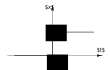
\includegraphics[width=0.4\linewidth]{signal-unit-step.png}
%\end{center}

\concept{Signo}

Se suele denotar como
\begin{equation*}
    \fx[\sgn]{t} =
    \left\{
    \begin{aligned}
        -1 \text{ si $t<0$ }
        \\
        1 \text{ si $t>0$ }
    \end{aligned}
    \right.
\end{equation*} 

En $t=0$ puede estar definida como -1, 1 o 0 según la aplicación.

%\begin{center}
%    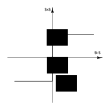
\includegraphics[width=0.4\linewidth]{signal-sgn.png}
%\end{center}

El escalón unitario y la función signo son \emph{funciones escalonadas}. Una función escalón es una función definida por una cantidad finita de tramos finitos que toman valores constantes. Ambas se relacionan de la siguiente forma.

\begin{mdframed}[style=MyFrame1]
    \begin{prop}
    \end{prop}
    \begin{equation*}
        \fx[u]{t} = \frac{\fx[sg]{t} + 1}{2}
    \end{equation*}
\end{mdframed}

\concept{Rampa unitaria}

Se suele denotar como $\fx[r]{t}$ y representa una señal que aumenta a tasa constante.

%\begin{center}
%    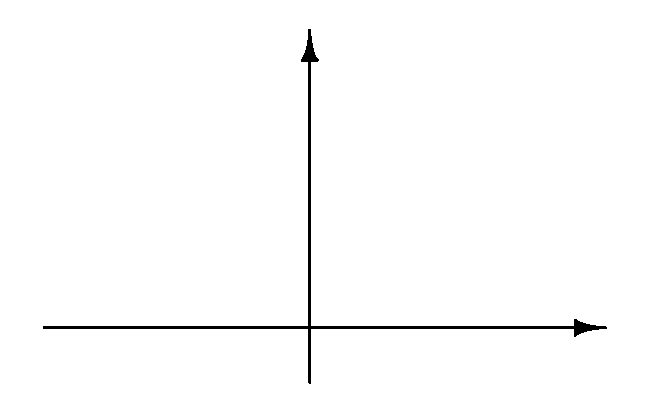
\includegraphics[width=0.4\linewidth]{signal-unit-ramp.png}
%\end{center}

Aquellas señales que se repiten cada cierto intervalo de tiempo $T$ son llamadas \emph{periódicas}. Estas son combinaciones lineales de las dadas anteriormente y a continuación se dan algunos ejemplos.

\concept{Tren de pulsos rectangulares y onda cuadrada}

Se suele denotar como
\begin{equation*}
    \fx[x]{t} = A \, \fx[\Pi]{\frac{t-t_0}{\tau}}
\end{equation*}

%\begin{center}
%    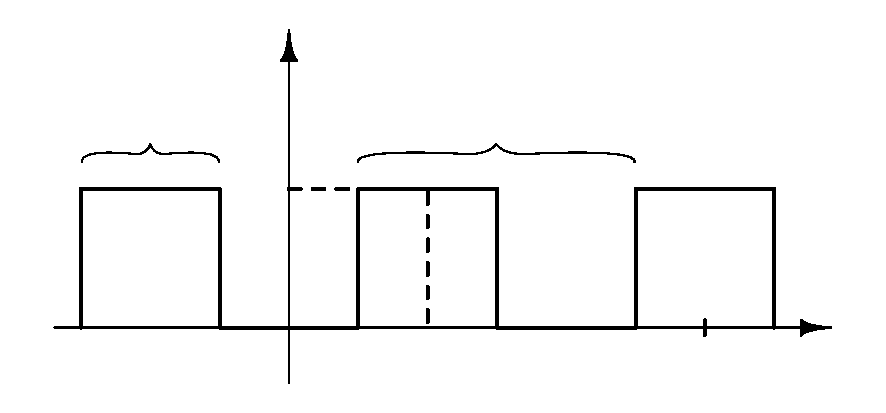
\includegraphics[width=0.6\linewidth]{signal-sq-wave.png}
%\end{center}

El valor pico es representado por $A$ ya que eventualmente vale 1 (como en el escalón unitario) pero puede estar escalada. También pueden darse corrimientos en tiempo según $t_0$ o desplazamientos del valor medio que la señal tome, en el eje vertical.

La relación entre el ancho ($\tau$) de los pulsos y el período ($T$) de la señal es llamada \emph{duty cycle}. En porcentajes se expresa:
\begin{equation*}
    \text{duty cycle}  \equiv \frac{\tau}{T} \cdot 100\%
\end{equation*}

Si esta relación es de 1:2 entonces el duty cycle es de $50\%$ y en tal caso el tren de pulsos se llama \emph{onda cuadrada}.

\concept{Tren de pulsos triangulares y onda triangular}

Se suele denotar como
\begin{equation*}
    \fx[x]{t} = A - \norm{t-t_0}
\end{equation*}

%\begin{center}
%    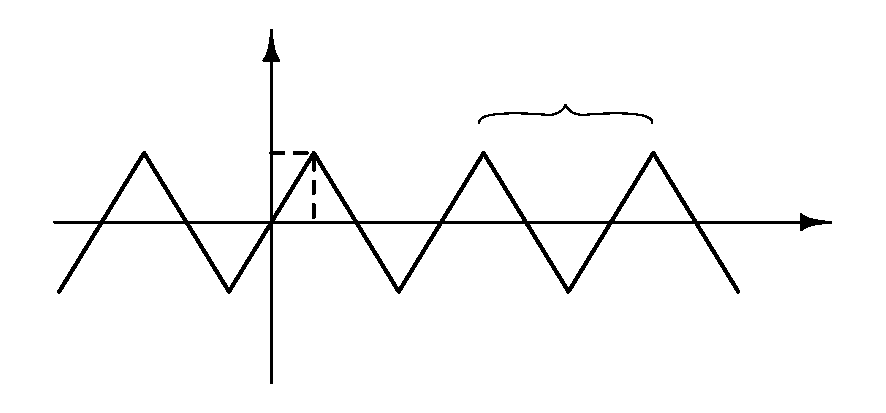
\includegraphics[width=0.6\linewidth]{signal-triang-wave.png}
%\end{center}

\concept{Diente de sierra}

%\begin{center}
%    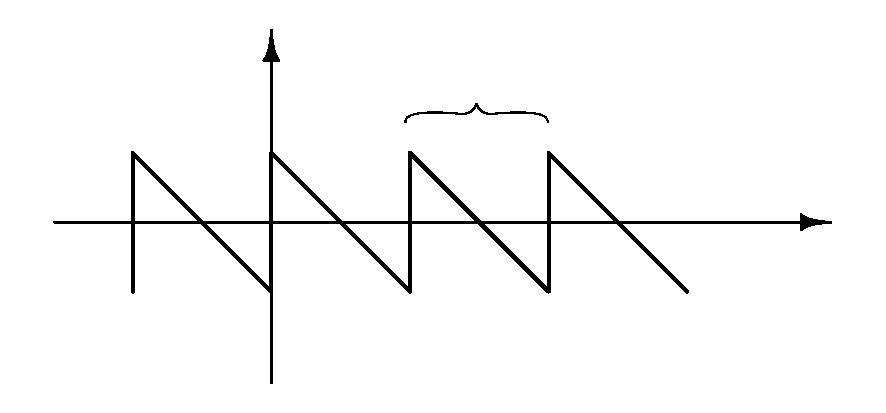
\includegraphics[width=0.6\linewidth]{signal-sawtooth.png}
%\end{center}

Observar, que el escalón unitario puede ser interpretado como la derivada de la rampa unitaria. Lo cual pareciera no tener sentido, porque la rampa pasa de tener una pendiente nula a una pendiente unitaria de manera no suave. Y efectivamente, en el sentido tradicional de la definición de derivada sería una interpretación errónea. Por este motivo el valor que el escalón toma en $t=0$ es arbitrario. Pero de igual manera es posible definir una función que sea la derivada del escalón unitario. En cero la función pasa de valer 0 a valer 1 abruptamente y no es posible definir la derivada en el sentido tradicional. Pero es posible dar una noción de derivada uniendo los dos tramos del escalón con una rampa que va ``desde la izquierda del cero hasta la derecha del cero'' para obtener una función continua.

%\begin{center}
%    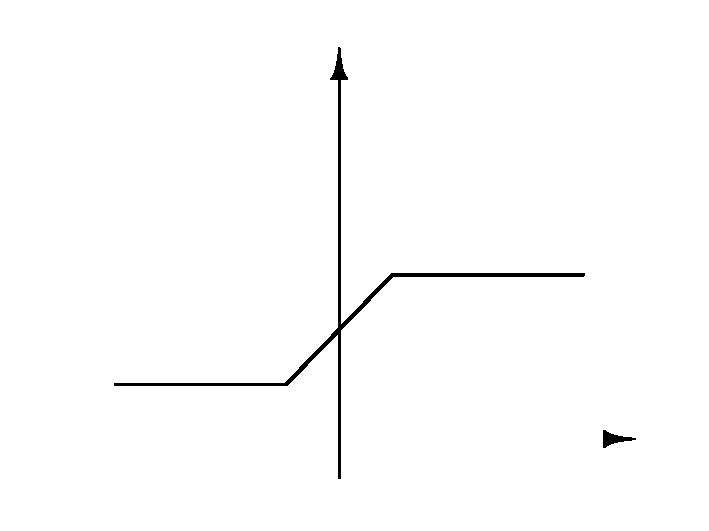
\includegraphics[width=0.4\linewidth]{signal-impulse-2.png}
%\end{center}

Personalmente, me gusta pensar que se trata de una función que tiene 2 dimensiones temporales: una en el sentido de $t$ y otra hacia ``adentro''. De manera que es posible que la función tenga un cambio ``suave'' y discontinuo simultáneamente para un único instante $t_0$, ya que el reloj no estaría frenándose sino que estaría usando otras manecillas.

Vemos que cuando el ``corte en cero'' tiende a unirse, la pendiente de la rampa que une ambos tramos es infinita, pues es una línea vertical. Este razonamiento corresponde a definir las señales a partir de lo que se conoce como \emph{funciones generalizadas}.

Las funciones generalizadas son objetos matemáticos que pretenden extender el concepto tradicional de función, para poder definir una noción de derivada para funciones que no son derivables. Fueron introducidas por Serguéi Sóbolev en 1935 y formalizadas en 1950 por Laurent Schwartz en su \emph{teoría de distribuciones}.

Las funciones tradicionales se definen con una asignación entre conjuntos y una fórmula, y el cálculo infinitesimal está dado por la integral de Riemann. En cambio, \textbf{a muy grandes rasgos}, una función generalizada se define como una función partida según el entorno de un punto. El estudio infinitesimal se hace a partir de un \emph{funcional}, para luego definir la función generalizada a partir del \emph{límite débil} del funcional.

\begin{mdframed}[style=MyFrame1]
    \begin{prop}
        \label{prop:limDebil}
    \end{prop}
    \cusTi{Límite débil de una distribución}
    \cusTe{Para un funcional $\fx{x}$ y una función continua de prueba $\fx[\phi]{x}$ se cumple que}
    \begin{equation*}
        \lim_{x \to 0} \int \fx{x-x_0} \, \fx[\phi]{x} \, \dif x = \fx[\phi]{x_0}
    \end{equation*}
\end{mdframed}


\concept{Delta de Dirac e impulso unitario}

Se suele denotar como
\begin{equation*}
    \fx[\delta]{t-t_0} =
    \left\{
    \begin{aligned}
        \infty \text{ si $t=t_0$ }
        \\
        0 \text{ si $t \neq t_0$ }
    \end{aligned}
    \right.
\end{equation*}

Y se la representa gráficamente con una flecha haciendo referencia a que en el punto $t_0$ la función toma, por un instante, un valor infinito. La \emph{altura} de la flecha indica el área ($\lambda$). Si la función tiene área unitaria, se la llama impulso unitario.

%\begin{center}
%    \includegraphics[width=0.4\linewidth]{signal-impulse.png}
%\end{center}

Los cuadrados grises representan el área de un pulso centrado en $t_0$, inicialmente de ancho $\tau$ y amplitud $\lambda / \tau$. El área es el producto de la base por la altura, dada en este caso por $\lambda$. Al tomar el límite $\tau \to 0$ vemos que el pulso tiende a ser un impulso, ya que se hace de ancho nulo y altura infinita manteniendo su área constante.

Esto se debe a que el pulso $\frac{\lambda}{\tau} \, \fx[\Pi]{\frac{t-t_0}{\tau}}$ es el funcional y verifica
\begin{equation*}
    \lim_{\tau \to 0} \frac{\lambda}{\tau} \, \fx[\Pi]{\frac{t-t_0}{\tau}} = \lambda \, \fx[\delta]{t-t_0}
\end{equation*}

Ahora bien, si un impulso es la derivada de un pulso, entonces la integral del impulso que corresponde a su área está dada por la propiedad \ref{prop:limDebil} como sigue.
\begin{equation*}
    \lim_{\tau \to 0} \int_{-\infty}^\infty \frac{\lambda}{\tau} \, \fx[\Pi]{\frac{t-t_0}{\tau}} \, \dif t
    = \int_{-\infty}^\infty \lambda \, \fx[\delta]{t-t_0} \, \dif t
    = \lambda
\end{equation*}

Es decir que para el caso del impulso unitario $\lambda = 1$ obteniendo la siguiente propiedad, a partir de la que se suele definir la delta de Dirac.

\begin{mdframed}[style=MyFrame1]
    \begin{prop}
    \end{prop}
    \begin{equation*}
        \int_{-\infty}^\infty \fx[\delta]{t} \, \dif t = 1
    \end{equation*}
\end{mdframed}

\begin{mdframed}[style=MyFrame2]
    \begin{example}
    \end{example}
    \cusTi{Densidad de un cuerpo puntual}
    \begin{formatI}
        En este ejemplo se propone una función generalizada para describir una situación física. Se pretende comprobar que se verifica la propiedad \ref{prop:limDebil}.
    \end{formatI}
    El volumen ($V$) de un cuerpo sólido de forma esférica y radio $r$ es
    \begin{equation*}
        V = \frac{4 \, \pi \, r^3}{3}
    \end{equation*}
    
    Si la masa ($m$) del cuerpo está uniformemente distribuída, su densidad ($\rho$) está dada por
    \begin{equation*}
        \rho = \frac{m}{V}
    \end{equation*}

    Por simplicidad, se supone que la masa del cuerpo es unitaria.
    
    De manera que se define una \emph{función generalizada} $\delta$ que a cada punto ($\Vec{x}$) del espacio le asigna la densidad en ese punto.
    \begin{equation*}
        \fx[\delta]{\Vec{x}} =
        \left\{
        \begin{aligned}
            \frac{3}{4 \, \pi \, r^3} \text{ si } \nnorm{\Vec{x}} \leq r
            \\
            0 \text{ si } \nnorm{\Vec{x}} > r
        \end{aligned}
        \right.
    \end{equation*}
            
    Suponer que el cuerpo sea puntual implica evaluar $r \to 0$ de manera que la densidad ($\delta$) queda dada por
    \begin{equation*}
        \fx[\delta]{\Vec{x}} =
        \left\{
        \begin{aligned}
            \infty \text{ si } \nnorm{\Vec{x}} = 0
            \\
            0 \text{ si } \nnorm{\Vec{x}} > 0
        \end{aligned}
        \right.
    \end{equation*}
    
    A partir del diferencial de masa, se obtiene la misma integrando miembro a miembro:
    \begin{gather*}
        \dif m = \fx[\delta]{\Vec{x}} \, \dif V
        \\
        m = \int \fx[\delta]{\Vec{x}} \, \dif V
    \end{gather*}

    En el volumen que encierra el cuerpo, la masa es unitaria por hipótesis. Pero para los puntos del espacio que no sean ocupados por el cuerpo, la masa es nula. Luego
    \begin{equation*}
        \int_V \fx[\delta]{\Vec{x}} \, \dif V =
        \left\{
        \begin{aligned}
            1 \text{ si } \nnorm{\Vec{x}} \in V
            \\
            0 \text{ si } \nnorm{\Vec{x}} \notin V
        \end{aligned}
        \right.
    \end{equation*}

    De manera que este es un ejemplo donde se cumple la propiedad \ref{prop:limDebil} para la función de prueba $\phi$ unitaria y $\Vec{x}_0$ en el origen. El funcional, en este caso, sería $\fx[\delta]{\Vec{x}}$ antes de tomar el límite cuando $r \to 0$.
\end{mdframed}


\section{Energía y potencia de señales}

\begin{align*}
        \sub{E}{tot} \text{ converge} & \implies \sub{P}{tot} \to 0
        \\
        \sub{P}{tot} \text{ converge} & \implies \sub{E}{tot} \to \infty
        \\
        \sub{P}{tot} \to \infty & \implies \sub{P}{tot} \to \infty
    \end{align*}

\begin{mdframed}[style=MyFrame1]
    \begin{defn}
    \end{defn}
    \cusTi{Energía de una señal}
    \begin{equation*}
        E = \int_{-\infty}^{\infty} \norm{\fx[x]{t}}^2 \dif t
    \end{equation*}
\end{mdframed}

\begin{mdframed}[style=MyFrame1]
    \begin{defn}
    \end{defn}
    \cusTi{Potencia de una señal}
    \begin{equation*}
        P = \lim_{\Delta t \to \infty} \frac{1}{\Delta t} \int_{-\frac{T}{2}}^{\frac{T}{2}} \norm{\fx[x]{t}}^2 \dif t
    \end{equation*}
\end{mdframed}


\section{Suma no correlacionada}

La suma de señales de diferente frecuencia puede ser expresada por
\begin{align*}
    \fx[x]{t} &= e^{\iu \omega_1 t} + e^{\iu \omega_2 t}
    \\
    &= e^{\iu \frac{\omega_1 + \omega_2}{2} t} \left( e^{\iu \omega_0 t} \pm e^{-\iu \omega_0 t} \right)
    \\
    &= \left\{
    \begin{aligned}
        2 \, e^{\iu \frac{\omega_1 + \omega_2}{2} t} \, \fx[\cos]{\omega_0 \, t}
        \\
        2 \, \iu \, e^{\iu \frac{\omega_1 + \omega_2}{2} t} \, \fx[\sin]{\omega_0 \, t}
    \end{aligned}
    \right.
    \\[1ex]
    \text{Donde } \frac{\omega_1+\omega_2}{2} \pm \omega_0 &=
    \left\{
    \begin{aligned}
        & \omega_1
        \\
        & \omega_2
    \end{aligned}
    \right.
\end{align*}


\section{Señales discretas}

\begin{mdframed}[style=MyFrame1]
    \begin{defn}
        \label{defn:funcDiscPeriod}
    \end{defn}
    \cusTi{Función discreta periódica}
    \cusTe{$x: \setZ \longrightarrow \setC$ es una función periódica si y solo si}
    \begin{equation*}
        x[n] = x[n+N]
    \end{equation*}
    \noTi{donde $N \in \setN$ es el período.}
\end{mdframed}

Sea $\Omega \in \setR$ la frecuencia angular, por definición se tiene
\begin{gather*}
    \left\{
    \begin{aligned}
        & x[n] = e^{\iu \Omega n}
        \\
        & x[n+N] = e^{\iu \Omega n} \, e^{\iu \Omega N}
    \end{aligned}
    \right.
    \\[1ex]
    e^{\iu \Omega n} = e^{\iu \Omega n} \, e^{\iu \Omega N}
    \\
    1 = e^{\iu \Omega N}
\end{gather*}

Y 1 puede ser expresado como un número complejo en su forma polar, quedando luego:
\begin{gather*}
    e^{\iu 2 k \pi} = e^{\iu \Omega N} \text{ con $k \in \setN$}
    \\
    \iu \, 2 \, k \, \pi = \iu \, \Omega \, N
    \\
    N = \frac{2 \, k \, \pi}{\Omega}
\end{gather*}

Pudiendo definir para $k=1$ el período fundamental
\begin{equation*}
    N_0 = \frac{2 \, \pi}{\Omega}
\end{equation*}

Observar que $2 \, k \in \setN \, \forall \, k$ pero, dado que se tiene que cumplir que $N \in \setN$ y $\Omega \in \setR$, para que una función discreta sea periódica se tiene que verificar que $\Omega$ sea múltiplo de $\pi$.

\begin{mdframed}[style=MyFrame1]
    \begin{prop}
    \end{prop}
    \begin{equation*}
        x[n] \text{ es periódica} \iff \frac{\pi}{\Omega} \in \setN
    \end{equation*}
\end{mdframed}

Además, si $N=1$ fuese un período válido, la función tomaría el mismo valor en todas las muestras. Y en tal caso $x[n] = x[n_\ith]$ para todo $n_\ith$ mientras que la implicancia en la definición \ref{defn:funcDiscPeriod} es en ambos sentidos. Con lo cual, se deduce que:

\begin{mdframed}[style=MyFrame1]
    \begin{prop}
    \end{prop}
    \noTi{El mínimo período es $N=2$ con lo cual $\Omega_0 = \pi$ es la máxima frecuencia.}
\end{mdframed}


\chapter{Caracterización de sistemas}

\begin{mdframed}[style=MyFrame1]
    \begin{defn}
    \end{defn}
    \cusTi{Sistema invariante en el tiempo}
    \cusTe{Un sistema es invariante en el tiempo si al excitarlo con $\fx[x]{t-t_0}$ genera $\fx[y]{t-t_0}$.}
\end{mdframed}

\begin{mdframed}[style=MyFrame1]
    \begin{defn}
    \end{defn}
    \cusTi{Sistema estable}
    \cusTe{Un sistema es estable si para una entrada acotada en amplitud, la salida también es acotada.}
\end{mdframed}

\begin{mdframed}[style=MyFrame1]
    \begin{defn}
    \end{defn}
    \cusTi{Sistema causal}
    \cusTe{Un sistema es causal o no anticipativo si la salida no comienza antes de aplicar la entrada.}
\end{mdframed}
 

\section{Función de transferencia}

\begin{mdframed}[style=MyFrame1]
    \begin{defn}
    \end{defn}
    \cusTi{Función de transferencia}
    \cusTe{Dados los espectros frecuenciales de las señales de entrada $\fx[X]{s}$ y salida $\fx[Y]{s}$ de un sistema, se define el cociente de estos como la función de transferencia del mismo.}
    \begin{equation*}
        \fx[H]{s} = \frac{\fx[Y]{s}}{\fx[X]{s}}
    \end{equation*}
\end{mdframed}

\begin{mdframed}[style=MyFrame1]
    \begin{prop}
    \end{prop}
    \noTi{Un sistema lineal e invariante en el tiempo excitado por una señal $\fx[x]{t} = A_x \fx[\cos]{\omega_x \, t + \varphi_x}$ presenta una señal de salida $\fx[y]{t} = A_y \fx[\cos]{\omega_y \, t + \varphi_y}$} tal que
    \begin{equation*}
        \fx[H]{\omega} = \frac{\fx[y]{\omega}}{\fx[x]{\omega}}
    \end{equation*}
\end{mdframed}

Considerando que $\fx[H]{\omega} = \norm{\fx[H]{\omega}} \, e^{\iu \fx[\arg]{\fx[H]{\omega}}}$ se puede demostrar la siguiente propiedad.

\begin{mdframed}[style=MyFrame1]
    \begin{prop}
    \end{prop}
    \begin{gather*}
        \norm{\fx[H]{\omega_x}} = \frac{A_y}{A_x}
        \\[1ex]
        \fx[\arg]{\fx[H]{\omega_x}} = \varphi_y - \varphi_x
    \end{gather*}
\end{mdframed}


\chapter{Convolución}


\begin{mdframed}[style=MyFrame1]
    \begin{defn}
    \end{defn}
    \cusTi{Respuesta al impulso}
    \cusTe{La respuesta al impulso de un sistema lineal e invariante en el tiempo, representado por una transformación $T$, es la señal de salida obtenida cuando este es excitado por una delta de Dirac como señal de entrada.}
    \begin{equation*}
        \fx[h]{t} = \fx[T]{\fx[\delta]{t}}
    \end{equation*}
\end{mdframed}

Tomando $\fx[\delta]{t-t_0}$ como un funcional para cualquier señal $\fx[x]{t}$ contínua, según la propiedad \ref{prop:limDebil}, se tiene
\begin{equation*}
    \int_{-\infty}^\infty \fx[\delta]{t-t_0} \, \fx[x]{t} \, \dif t = \fx[x]{t_0}
\end{equation*}

Y renombrando la variable de integración queda
\begin{equation*}
    \int_{-\infty}^\infty \fx[\delta]{\tau-t_0} \, \fx[x]{\tau} \, \dif \tau = \fx[x]{t_0}
\end{equation*}

Dado que $\fx[\delta]{t} = \fx[\delta]{-t}$ para cualquier $t=t_0$ genérico
\begin{equation*}
    \fx[x]{t} = \int_{-\infty}^\infty \fx[\delta]{t-\tau} \, \fx[x]{\tau} \, \dif \tau
\end{equation*}

Sea $T$ una transformación dada por un sistema lineal e invariante en el tiempo.

Al excitar el sistema con $\fx[x]{t}$ como señal de entrada se obtiene $\fx[y]{t} = \fx[T]{\fx[x]{t}}$ como salida. Y al aplicar $T$ queda
\begin{equation*}
    \fx[y]{t} = \fx[T]{ \int_{-\infty}^\infty \fx[\delta]{t-\tau} \, \fx[x]{\tau} \, \dif \tau }
\end{equation*}

que por linealidad es
\begin{equation*}
    \fx[y]{t} = \int_{-\infty}^\infty \fx[T]{\fx[\delta]{t-\tau}} \, \fx[x]{\tau} \, \dif \tau
\end{equation*}

y por invarianza en el tiempo $\fx[T]{\fx[\delta]{t-\tau}}$ es la respuesta al impulso, obteniendo la que se conoce como integral de convolución.

\begin{mdframed}[style=MyFrame1]
    \begin{defn}
    \end{defn}
    \cusTi{Integral de convolución}
    \begin{equation*}
        \fx[x]{t} * \fx[h]{t} = \int_{-\infty}^\infty \fx[x]{\tau} \, \fx[h]{t-\tau} \, \dif \tau
    \end{equation*}
\end{mdframed}

Esta operación implica que la salida de un sistema LTI es la \emph{convolución} entre su respuesta al impulso y la señal de entrada.

\begin{mdframed}[style=MyFrame1]
    \begin{prop}
    \end{prop}
    \cusTi{Respuesta al impulso}
    \begin{equation*}
        \fx[y]{t} = \fx[h]{t} * \fx[x]{t}
    \end{equation*}
\end{mdframed}

A continuación se tiene un esquema que representa gráficamente esta interpretación.

%\begin{center}
%    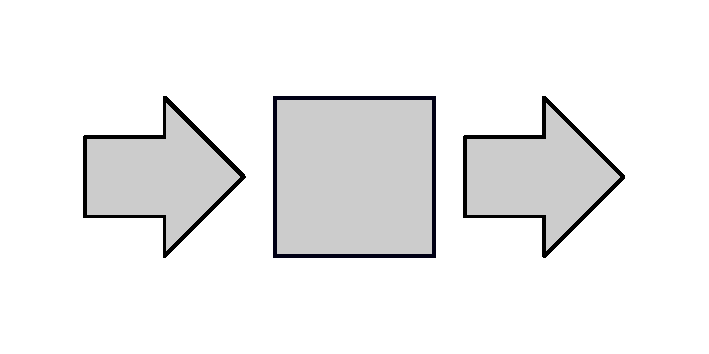
\includegraphics[width=0.4\linewidth]{system.png}
%\end{center}


\chapter{Transformada de Fourier}


\section{Serie de Fourier}

Una función $\fx[x]{t}$ de período fundamental $T_0 = \frac{2 \, \pi}{\omega_0}$ tiene desarrollo de Fourier si cumple las \emph{condiciones de Dirichlet}:
\begin{itemize}
    \item Es absolutamente inegrable: $\int_{T_0} \norm{\fx[x]{t}} \, \dif t < \infty$
    \item Tiene una cantidad finita de máximos y mínimos en $T_0$
    \item Tiene una cantidad finita de discontinuidades en $T_0$
\end{itemize}

\begin{mdframed}[style=MyFrame1]
    \begin{defn}
        \label{defn:FourierSerieExp}
    \end{defn}
    \cusTi{Serie de Fourier: forma exponencial compleja}
    \begin{equation*}
        \fx[x]{t} = \sum_{\kth=-\infty}^\infty c_\kth \, e^{\iu \, \kth \, \omega_0 \, t}
    \end{equation*}
    \noTi{donde $c_\kth$ son los coeficientes de Fourier complejos dados por}
    \begin{equation*}
        c_\kth = \frac{1}{T_0} \int_{T_0} \fx[x]{t} \, e^{-\iu \, \kth \, \omega_0 \, t} \, \dif t
    \end{equation*}
\end{mdframed}

Reacomodando la sumatoria de la definición \ref{defn:FourierSerieExp} como sigue
\begin{align*}
    \fx[x]{t} &=
    \sum_{\kth=-\infty}^\infty c_\kth \, e^{\iu \, \kth \, \omega_0 \, t}
    \\[1em]
    &= \sum_{\kth=-\infty}^{-1} c_\kth \, e^{\iu \, \kth \, \omega_0 \, t} + c_0 + \sum_{\kth=1}^{\infty} c_\kth \, e^{\iu \, \kth \, \omega_0 \, t}
    \\[1em]
    &= \sum_{\kth=1}^{\infty} c_{-\kth} \, e^{-\iu \, \kth \, \omega_0 \, t} + c_0 + \sum_{\kth=1}^{\infty} c_\kth \, e^{\iu \, \kth \, \omega_0 \, t}
\end{align*}

es posible obtener la siguiente expresión equivalente:
\begin{equation}
    \fx[x]{t} = c_0 + \sum_{\kth=1}^{\infty} \bb{ c_\kth \, e^{\iu \, \kth \, \omega_0 \, t} + c_{-\kth} \, e^{-\iu \, \kth \, \omega_0 \, t} }
    \label{eqn:FourierExpBis}
\end{equation}

Y aplicando la fórmula de Euler:
\begin{align*}
    &
    \scale{0.80}{
    = c_0 + \sum_{\kth=1}^{\infty} \braces{c_\kth \sqb{\fx[\cos]{\kth \, \omega_0 \, t} + \iu \fx[\sin]{\kth \, \omega_0 \, t}} + c_{-\kth} \sqb{\fx[\cos]{\kth \, \omega_0 \, t} - \iu \fx[\sin]{\kth \, \omega_0 \, t}} }
    }
    \\[1em]
    &= c_0 + \sum_{\kth=1}^{\infty} \sqb{ \bb{c_\kth + c_{-\kth}} \fx[\cos]{\kth \, \omega_0 \, t} + \iu \bb{c_\kth - c_{-\kth}} \fx[\sin]{\kth \, \omega_0 \, t} }
\end{align*}

\begin{mdframed}[style=MyFrame1]
    \begin{defn}
        \label{defn:FourierSerieTrig}
    \end{defn}
    \cusTi{Serie de Fourier: forma trigonométrica}
    \begin{equation*}
        \fx[x]{t} = c_0 + \sum_{\kth=1}^{\infty} \sqb{a_\kth \fx[\cos]{\kth \, \omega_0 \, t} + b_\kth \fx[\sin]{\kth \, \omega_0 \, t} }
    \end{equation*}
    \noTi{donde $a_\kth = c_\kth + c_{-\kth}$ y $b_\kth = \iu \bb{c_\kth - c_{-\kth}}$ son los coeficientes de Fourier trigonométricos.}
\end{mdframed}

Por otro lado, si se aplica la fórmula de Euler pero esta vez en la exponencial de los coeficientes complejos de la definición \ref{defn:FourierSerieExp}:
\begin{align*}
    c_{\pm\kth} &= \frac{1}{T_0} \int_{T_0} \fx[x]{t} \, e^{\mp \iu \, \kth \, \omega_0 \, t} \, \dif t
    \\
    &= \frac{1}{T_0} \int_{T_0} \fx[x]{t} \sqb{ \fx[\cos]{\kth \, \omega_0 \, t} \mp \iu \fx[\sin]{\kth \, \omega_0 \, t} } \, \dif t
    \\
    &= \frac{1}{T_0} \int_{T_0} \fx[x]{t} \fx[\cos]{\kth \, \omega_0 \, t} \dif t
    \mp \frac{\iu}{T_0} \int_{T_0} \fx[x]{t} \fx[\sin]{\kth \, \omega_0 \, t} \dif t
\end{align*}

Se definen los términos $\alpha = \int_{T_0} \fx[x]{t} \fx[\cos]{\kth \, \omega_0 \, t} \dif t$ y $\beta = \int_{T_0} \fx[x]{t} \fx[\sin]{\kth \, \omega_0 \, t} \dif t$ para simplificar la notación, tal que:
\begin{equation*}
     c_{\pm\kth} = \frac{\alpha}{T_0} \mp \iu \frac{\beta}{T_0}
\end{equation*}

Obteniendo las siguientes expresiones para los coeficientes trigonométricos de la definición \ref{defn:FourierSerieTrig}:
\begin{equation*}
    \left\{
    \begin{aligned}
        a_\kth &= c_\kth + c_{-\kth} = \frac{2 \, \alpha}{T_0}
        \\
        b_\kth &= \iu \bb{c_\kth - c_{-\kth}} = \frac{2 \, \beta}{T_0}
    \end{aligned}
    \right.
\end{equation*}

Esto no es casualidad y viene dado por una propiedad que sale de sumar complejos conjugados. Podemos comprobarla gráficamente. Dado que $a_\kth \in \setR$ y $b_\kth \in \setI$ son ortogonales entre sí, los coeficientes $c_{\pm\kth} \in \setC$ no forman cualquier ángulo, sino que $c_\kth$ es el conjugado de $c_{-\kth}$. A continuación se muestran con flechas en el plano complejo:

%\begin{center}
%    \includegraphics[width=0.5\linewidth]{abc.png}
%\end{center}

A partir del gráfico anterior, se define el complejo $C_\kth = a_\kth - \iu \, b_\kth$ representado por un punto en el vértice del triángulo gris.

Luego, multiplicando y dividiendo por $\norm{C_\kth}$ la serie de la definición \ref{defn:FourierSerieTrig} se tiene
\begin{equation*}
    \fx[x]{t} = c_0 + \sum_{\kth=1}^{\infty} \norm{C_\kth} \sqb{ \dfrac{a_\kth}{\norm{C_\kth}} \fx[\cos]{\kth \, \omega_0 \, t} + \dfrac{b_\kth}{\norm{C_\kth}} \fx[\sin]{\kth \, \omega_0 \, t} }
\end{equation*}

Por trigonometría se tiene $\fx[\cos]{\theta_\kth} = a_\kth / \norm{C_\kth}$ mientras que $\fx[\sin]{\theta_\kth} = b_\kth / \norm{C_\kth}$ luego:
\begin{equation*}
    \fx[x]{t} = c_0 + \sum_{\kth=1}^{\infty} \norm{C_\kth} \sqb{ \fx[\cos]{\theta_\kth} \fx[\cos]{\kth \, \omega_0 \, t} + \fx[\sin]{\theta_\kth} \fx[\sin]{\kth \, \omega_0 \, t} }
\end{equation*}

Aplicando $\fx[\cos]{\alpha \pm \beta} = \fx[\cos]{\alpha} \fx[\cos]{\beta} \mp \fx[\sin]{\alpha} \fx[\sin]{\beta}$ se infiere:

\begin{mdframed}[style=MyFrame1]
    \begin{defn}
        \label{defn:FourierSerieArm}
    \end{defn}
    \cusTi{Serie de Fourier: forma armónica}
    \begin{equation*}
        \fx[x]{t} = c_0 + \sum_{\kth=1}^{\infty} \norm{C_\kth} \fx[\cos]{\kth \, \omega_0 \, t - \theta_\kth}
    \end{equation*}
    \noTi{donde $C_\kth$ son los coeficientes de Fourier expresados en forma polar, tal que:}
    \begin{equation*}
    \left\{
    \begin{aligned}
        \norm{C_\kth} = \sqrt{a_\kth^2 + b_\kth^2}
        \\
        \theta_\kth = \fx[\artan]{\frac{b_\kth}{a_\kth}}
    \end{aligned}
    \right.
\end{equation*}
\end{mdframed}

\begin{mdframed}[style=MyFrame2]
    \begin{example}
    \end{example}
    \cusTi{De la proyección ortogonal a la serie}
    \begin{formatI}
        Calcular la proyección ortogonal de una onda cuadrada. Obtener los coeficientes de Fourier complejos. Demostrar que son equivalentes a una serie deducida a partir de la proyección.
    \end{formatI}
    \vspace{1em}
    Sea $x$ una función por partes dada por
    \begin{equation*}
        \fx[x]{t} =
        \left\{
        \begin{matrix}
            0 & \text{si } -\pi < t < -\frac{\pi}{2}
            \\
            1 & \text{si } -\frac{\pi}{2} < t < \frac{\pi}{2}
            \\
            0 & \text{si } \frac{\pi}{2} < t < \pi
        \end{matrix}
        \right.
    \end{equation*}
    
    Sea $B_S$ una base de polinomios trigonométricos. A saber:
    \begin{equation*}
        B_S = \braces{1; \fx[\sin]{t}; \fx[\cos]{t}; \fx[\sin]{2t}; \dots; \fx[\sin]{\kth t}; \fx[\cos]{\kth t}}
    \end{equation*}
    
    De manera que la proyección de $x$ sobre $S$ es:
    \begin{multline*}
        \fx[\proy_S]{x} =
        \\
        = \frac{1}{2} + \frac{2}{\pi} \sqb{\fx[\cos]{t} - \dfrac{\fx[\cos]{3t}}{3} + \dfrac{\fx[\cos]{5t}}{5} - \dfrac{\fx[\cos]{7t}}{7} \cdots}
    \end{multline*}

    Y puede ser expresada por la siguiente serie:
    \begin{equation}
        \fx[\proy_S]{x} = \frac{1}{2} + \frac{2}{\pi} \sum_{\kth=1}^\infty \frac{\bb{-1}^{\kth+1}}{2 \, \kth - 1} \, \ffx[\cos]{\bb{2 \, \kth -1} t}
        \label{eqn:FourierProy}
    \end{equation}

    Para un pulso rectangular genérico
    \begin{equation*}
        \fx[x]{t} = A \, \fx[\Pi]{\frac{t-t_0}{\tau}}
    \end{equation*}
    
    los coeficientes están dados según la definición \ref{defn:FourierSerieExp} como sigue:
    \begin{align*}
        c_\kth &= \frac{1}{T_0} \int_{T_0} \fx[x]{t} \, e^{-\iu \, \kth \, \omega_0 \, t} \, \dif t
        \\[1ex]
        &= \frac{A}{T_0} \int_{-\frac{\tau}{2}}^{\frac{\tau}{2}} e^{-\iu \, \kth \, \omega_0 \, t} \, \dif t
        \\[1ex]
        &= \frac{A}{T_0} \barrow{\dfrac{e^{-\iu \, \kth \, \omega_0 \, t}}{-\iu \, \kth \, \omega_0}}{-\frac{\tau}{2}}{\frac{\tau}{2}}
        \\[1ex]
        &= \frac{A}{-2 \, \pi \, \iu \, \kth } \bb{ e^{ -\iu \, \omega_0 \, \kth \frac{\tau}{2}} - e^{ \iu \, \omega_0 \, \kth \frac{\tau}{2}} }
        \\[1ex]
        &= \frac{A}{\pi \, \kth} \, \fx[\sin]{\frac{\omega_0 \, \kth \, \tau}{2}}
        \\[1ex]
        &= \frac{A}{\pi \, \kth} \, \fx[\sin]{\frac{\pi \, \kth \, \tau}{T_0}}
        \\[1ex]
        &= \frac{A \, \tau}{T_0} \cdot
        \frac{ \fx[\sin]{\dfrac{\pi \, \kth \, \tau}{T_0}} }{ \dfrac{\pi \, \kth \, \tau}{T_0} }
    \end{align*}

    Esto es
    \begin{equation*}
        c_\kth = \frac{A \, \tau}{T_0} \, \fx[\sinc]{\frac{\pi \, \kth \, \tau}{T_0}}
    \end{equation*}

    Particularmente si $A=1$, $T_0=2\,\pi$, $\tau=\pi$ queda
    \begin{equation*}
        c_\kth = \frac{ \fx[\sin]{\frac{\kth \, \pi}{2}} }{\kth \, \pi}
    \end{equation*}

    Según la ecuación \ref{eqn:FourierExpBis} se tiene:
    \begin{align*}
        \fx[x]{t} &= c_0 + \sum_{\kth=1}^{\infty} \bb{ c_\kth \, e^{\iu \, \kth \, \omega_0 \, t} + c_{-\kth} \, e^{-\iu \, \kth \, \omega_0 \, t} }
        \\
        &= c_0 + \sum_{\kth=1}^{\infty} \frac{\fx[\sin]{\frac{\kth \, \pi}{2}}}{\kth \, \pi} \bb{ e^{\iu \, \kth \, \omega_0 \, t} + e^{-\iu \, \kth \, \omega_0 \, t} }
    \end{align*}

    Obteniendo el desarrollo en series de Fourier para una onda cuadrada:
    \begin{equation*}
        \fx[x]{t} = c_0 + 2 \sum_{\kth=1}^{\infty} \frac{\fx[\sin]{\frac{\kth \, \pi}{2}}}{\kth \, \pi} \, \fx[\cos]{\kth \, \omega_0 \, t}
    \end{equation*}

    Observar que este desarrollo es equivalente a la ecuación \ref{eqn:FourierProy}, ya que $\fx[\sin]{\frac{\kth \, \pi}{2}}$ vale 0 para los $\kth$ pares y $\pm1$ para los $\kth$ impares.
\end{mdframed}

\begin{mdframed}[style=MyFrame1]
    \begin{prop}
    \end{prop}
    Los coeficientes $c_\kth^\nth$ de la serie de Fourier de la n-ésima derivada están dados por
    \begin{equation*}
        c_\kth^\nth = c_\kth \cdot \bb{\frac{\iu \, 2 \, \pi \, \kth}{T_0}}^\nth
    \end{equation*}
\end{mdframed}


\section{Transformada de Fourier}

Para una función $\fx[x]{t}$ real, el coeficiente complejo $c_0$ resulta ser el valor promedio de la misma:
\begin{equation*}
    c_0 = \frac{1}{T_0} \int_{T_0} \fx[x]{t} \, \dif t
\end{equation*}

Si se reemplaza $\fx[x]{t}$ por su desarrollo en serie (Def. \ref{defn:FourierSerieExp}), se obtiene:
\begin{align*}
    c_0 &= \frac{1}{T_0} \int_{T_0} \bb{\sum_{\kth=-\infty}^\infty c_\kth \, e^{\iu \, \kth \, \omega_0 \, t}} \dif t
    \\[1ex]
    &= \frac{1}{T_0} \int_{T_0} \sqb{\dots c_{-1} \, e^{\iu \bb{-1} \, \omega_0 \, t} + c_0 \, e^0 + c_1 \, \, e^{\iu \bb{1} \, \omega_0 \, t} \dots} \dif t
    \\[1ex]
    &= \dots \frac{1}{T_0} \int_{T_0} c_{-1} \, e^{\iu \bb{-1} \, \omega_0 \, t} \dif t
    + c_0
    + \frac{1}{T_0} \int_{T_0} c_1 \, \, e^{\iu \bb{1} \, \omega_0 \, t} \dif t \dots
\end{align*}

Poniéndose en evidencia que la única integral no nula es $\frac{1}{T_0} \int_{T_0} c_0 \, e^0 \, \dif t = c_0$. Las demás son integrales de funciones periódicas evaluadas en un período, como $\int_0^{2\pi} \fx[\sin]{t} \, \dif t = 0$.

Multiplicando el término $e^{-\iu \, 2 \, \pi \, \kth \, t}$ se consigue anular el promedio de cualquier integral que no sea $\omega_\kth=2 \, \pi \, \kth$ en general, particularmente de $\omega=0$ cuando $\kth=0$.

Así, es posible obtener cualquier coeficiente de Fourier:
\begin{equation*}
    \scale{0.98}{
    c_\kth = \frac{1}{T_0} \int_{T_0} \sqb{\dots c_{-1} \, e^{\iu \bb{-1} \, \omega_0 \, t} + c_0 \, e^0 + c_1 \, \, e^{\iu \bb{1} \, \omega_0 \, t} \dots} e^{-\iu \, 2 \, \pi \, \kth \, t} \dif t
    }
\end{equation*}

% Relacionar X con los coeficientes

\begin{mdframed}[style=MyFrame1]
    \begin{defn}
        \label{defn:FourierTrans}
    \end{defn}
    \cusTi{Transformada de Fourier}
    \begin{equation*}
        \fx[X]{\omega} = \int_{-\infty}^\infty \fx[x]{t} \, e^{-\iu \, \omega \, t} \, \dif t
    \end{equation*}
\end{mdframed}

\begin{mdframed}[style=MyFrame1]
    \begin{defn}
        \label{defn:FourierTrans}
    \end{defn}
    \cusTi{Transformada de Fourier inversa}
    \begin{equation*}
        \fx[x]{t} = \frac{1}{T_0} \int_{-\infty}^\infty \fx[X]{\omega} \, e^{\iu \, \omega \, t} \, \dif \omega
    \end{equation*}
\end{mdframed}

\begin{mdframed}[style=MyFrame2]
    \begin{example}
    \end{example}
    \cusTi{Espectro bipolar y forma de onda}
    \begin{equation*}
        \fx[x]{t} = 5 \fx[\sin]{2 \, \pi \, \SI{2}{\hertz} \, t + \pi} + 7 \fx[\sin]{2 \, \pi \, \SI{3}{\hertz} \, t - \pi/2}
    \end{equation*}
    %\begin{center}
    %    \includegraphics[width=0.5\linewidth]{spec-vs-wave-1.png}
    %\end{center}
    %\begin{center}
    %    \includegraphics[width=0.5\linewidth]{spec-vs-wave-2.png}
    %\end{center}
    %\begin{center}
    %    \includegraphics[width=0.5\linewidth]{spec-vs-wave-3.png}
    %\end{center}
    
\end{mdframed}




\end{document}
